
\documentclass[conference]{IEEEtran}
\IEEEoverridecommandlockouts
% MILCOM 2026 -- Track 4 (Integrated Network Architecture and Systems-of-systems).
\usepackage{cite}
\usepackage{amsmath,amssymb,amsfonts,amsthm}
\usepackage{algorithm}
\usepackage{algorithmic}
\usepackage{graphicx}
\usepackage{textcomp}
\usepackage{xcolor}
\usepackage{tikz}
\usetikzlibrary{arrows.meta,positioning,shapes.geometric,calc,backgrounds,fit}
\usepackage{booktabs}
\usepackage{array}
\usepackage{url}
\usepackage{balance}
\def\BibTeX{{\rm B\kern-.05em{\sc i\kern-.025em b}\kern-.08em
    T\kern-.1667em\lower.7ex\hbox{E}\kern-.125emX}}
\DeclareMathOperator*{\argmax}{arg\,max}
\DeclareMathOperator*{\argmin}{arg\,min}
\newtheorem{lemma}{Lemma}
\newtheorem{theorem}{Theorem}

\begin{document}

\title{Age-of-Secret Routing for Hybrid Quantum-Classical Tactical
       Non-Terrestrial Networks}

\author{\IEEEauthorblockN{Liang Dong}
\IEEEauthorblockA{\textit{Department of Electrical and Computer Engineering} \\
\textit{Baylor University}, Waco, Texas 76798, USA \\
Liang\_Dong@baylor.edu}}

\maketitle

\begin{abstract}
Tactical non-terrestrial networks (NTNs) combine satellites, airborne
relays, and ground stations whose cryptographic state can change as
fast as the radio state: a satellite pass ends, a gateway is blocked
by weather, a key pool runs dry, or a relay is policy-revoked.  We
introduce \emph{Age of Secret} (AoS), a routing-layer metric for
cryptographic freshness and key-pool depletion risk, analogous to
Age-of-Information but applied to keys rather than data, and prove
that the AoS-aware backpressure scheduler is throughput-optimal: the
joint queue and key-deficit process is mean-rate stable for every
arrival vector strictly inside a \emph{secure capacity region}
$\Lambda_S$ that we characterize.  We instantiate the framework in a
discrete-event NTN simulator driven by a current public TLE snapshot
of the real Starlink Phase-1 shell (1306 LEO satellites at
inclination 52.5--53.5\,$^\circ$ and altitude 530--570\,km, May 2026
epoch from CelesTrak/Space-Track), real-orbit pass-window propagation
via SGP4, a physically-grounded cloud-attenuation model fit to ISCCP
mid-latitude cloud climatology, and post-quantum cryptography
overheads at the ML-KEM throughput point.  Across five
seeds and five tactical scenarios (nominal, weather, relay
compromise, traffic surge, coalition partition), AoS-aware
backpressure attains \textbf{the lowest mean AoS in every scenario}
(2.5--29\,s) while matching the secure goodput of the best
unprincipled baseline; the closest competitor's mean AoS is
\textbf{1.8--11.6$\times$} higher.  We additionally implement the
ideal per-edge max-weight backpressure scheduler that
Theorem~\ref{thm:stab} covers directly, and verify empirically that
its joint queue and key-deficit Lyapunov function remains bounded.
Code and data sufficient to reproduce every reported number are
released with the paper.
\end{abstract}

\begin{IEEEkeywords}
Non-terrestrial networks, SATCOM, quantum networks, post-quantum
cryptography, secure routing, key management, Age of Secret, hybrid
trust plane, backpressure, tactical communications.
\end{IEEEkeywords}

\section{Introduction}
\label{sec:intro}
Tactical non-terrestrial networks integrate ground stations, gateways,
airborne relays, high-altitude platforms, and large LEO constellations
into a single resilient system of systems \cite{3gpp_ntn_overview}.
At the same time, long-term cryptographic risk is changing: quantum
computers threaten widely deployed public-key schemes, NIST has
standardized ML-KEM, ML-DSA, and SLH-DSA as the post-quantum
baseline~\cite{nist_fips203_2024,nist_fips204_2024,nist_fips205_2024},
and satellite quantum key distribution (QKD) has demonstrated
long-distance key generation in space-to-ground
links~\cite{liao_satellite_qkd_2017,pirandola_qkd_2020}.  Yet quantum
links are not magic secure networks: they require an authenticated
classical channel, are intermittent because of pointing, weather and
orbital pass windows, and do not solve routing, scheduling, or
denial-of-service problems~\cite{rfc9340_2023}.

This paper asks a practical operational question: how should a
tactical NTN route traffic when key material is a scarce, time-varying
network resource rather than a precomputed cryptographic detail?  We
introduce \emph{Age of Secret} (AoS), a routing-layer metric for
cryptographic freshness and key-pool depletion risk, analogous to
Age-of-Information~\cite{kaul_aoi_2012} but applied to keys.  AoS
quantifies whether a path has recent key material, sufficient
key-pool reserve, and acceptable trust state, without exposing the
secret key values themselves.

We then prove that an AoS-aware backpressure scheduler is
\emph{throughput-optimal} for the joint packet-and-key process: for
any arrival vector strictly inside a secure capacity region
$\Lambda_S$ defined by the average key-refresh rates, the joint
queue and key-deficit process is mean-rate stable.  The proof
extends Tassiulas--Neely
backpressure~\cite{tassiulas_backpressure_1992,neely_book_2010} into
the cryptographic-state domain by adding a key-deficit Lyapunov term.

The framework is validated in a discrete-event NTN simulator driven
by a \emph{current public TLE snapshot of the real Starlink Phase-1
shell}~\cite{celestrak_gp}: 1306 LEO satellites at
$52.5$--$53.5^\circ$ inclination and $530$--$570$~km altitude,
extracted from the May 2026 CelesTrak/Space-Track catalog by orbital
filtering, and propagated via SGP4.  Per-pass optical attenuation
follows a Beer--Lambert model parametrized by ISCCP-derived
mid-latitude cloud
climatology~\cite{rossow_schiffer_1999,itu_r_p1814}; the QKD
peak rate is calibrated to the published Micius BB84
measurements~\cite{liao_satellite_qkd_2017}; the PQC refresh rate is
set at the public liboqs ML-KEM-768 throughput
point~\cite{liboqs_2020} on a single CPU core.  Six tactical-edge
ground stations carry five flows across three security classes.
Across five seeds and five adversarial / degraded scenarios,
AoS-aware backpressure attains the lowest mean AoS in every scenario
while matching the secure goodput of the best unprincipled baseline.
All code and data are released at
\url{https://github.com/ProfessorDong/AoS-Routing}.

\section{System and Threat Model}
\label{sec:model}

\subsection{Network Model}
We model the tactical NTN as a discrete-time directed graph
$G(t)=(V,E(t))$ whose vertices include ground stations, regional
gateways, and LEO satellites, and whose edges represent the active
classical and quantum links at time $t$.  Each edge $e\in E(t)$
carries a classical capacity $C_e$ (bits/sec), a propagation latency
$L_e$, and a cryptographic \emph{key pool} $K_e(t)$ measured in
usable session-key bits.  Using a fixed step length $\Delta t\!=\!1$~s
throughout, the per-cycle dynamics are
\begin{equation}
 K_e(t{+}1)
 \;=\; \min\!\left\{K_e^{\max},\;
        \bigl[K_e(t) + G_e(t) - U_e(t)\bigr]^{+}\right\},
 \label{eq:keypool}
\end{equation}
where $[x]^{+}\!\triangleq\!\max\{x,0\}$ enforces non-negativity,
$G_e(t)\!\ge\!0$ is the per-cycle key inflow (PQC refresh plus QKD
generation when an overhead pass is in progress), $U_e(t)\!\ge\!0$
is the key consumption by protected traffic (key-bits per cycle),
and $K_e^{\min}$ is a policy reserve.  The scheduler is required to
respect $U_e(t)\!\le\!K_e(t)$ at every cycle, so $[\cdot]^{+}$ is in
fact attained without truncation under any valid schedule.  Each flow
$f\in\mathcal{F}$ has a source-destination pair, an arrival rate
$\lambda^f$ bits/sec (with mean-bounded second moment), a security
class $c_f$, and a freshness target $A_f^{\max}$; $Q^f_v(t)$ denotes
the bit-queue at vertex $v$ holding flow-$f$ data awaiting
transmission.  The induced \emph{secure capacity region} $\Lambda_S$
of supportable arrival vectors is characterized formally as a
polytope in Section~\ref{sec:algo}, jointly constrained by classical
link capacities and the time-average key-refresh rate $\bar G_e$.

\subsection{Age of Secret}
For an edge $e$, the local Age of Secret is
\begin{equation}
\mathrm{AoS}_e(t) = t - g_e(t) + \lambda_a \min\!\left\{\tau_d,\,
                    \tfrac{u_e(t)}{K_e(t)+\varepsilon}\right\}
                  + \mu_a R_e(t),
\label{eq:aos}
\end{equation}
where $g_e(t)$ is the generation time of the currently active key
epoch on $e$; $u_e(t)$ is the forecast \emph{per-cycle} key
consumption (in key-bits, the same unit as $K_e$), so the ratio
$u_e/(K_e{+}\varepsilon)$ and the cap $\tau_d$ are dimensionless;
$R_e(t)\in[0,1]$ is a trust/relay-risk score; and the policy weights
$\lambda_a,\mu_a$ are in seconds, giving the entire expression units
of time.  A path $P$ inherits the worst-edge value
$\mathrm{AoS}_P(t) = \max_{e \in P} \mathrm{AoS}_e(t)$.

\subsection{Threat Model}
A computationally-bounded adversary may inject interference along QKD
optical/RF channels, request the maximum admissible per-class traffic
to drain key pools, compromise one xApp or relay node and force a
geometric detour, or partition coalition gateways.  The adversary
\emph{cannot} break standardized PQC primitives
\cite{nist_fips203_2024,nist_fips204_2024,nist_fips205_2024} and
\emph{cannot} forge signed key-pool advertisements.  The defender
maintains signed AoS state, time-stamped nonces against replay, and
a signed policy bundle enumerating the admissible relays per class.

\section{AoS-Aware Backpressure: Theorem and Algorithm}
\label{sec:algo}

This section presents the analytical centerpiece of the paper.  We
state an AoS-aware backpressure weight rule together with the
\emph{ideal} per-edge max-weight scheduler it induces, characterise
the secure capacity region $\Lambda_S$ as a polytope, prove
mean-rate stability of the joint queue-and-key-deficit process under
a virtual-key-queue formulation, and then describe a tractable
per-flow Dijkstra implementation that is the Lagrangian-smoothed
approximation we actually deploy in the simulator.

\subsection{Per-Cycle Weight, Ideal Scheduler, and Region}

At each cycle $t$ the scheduler maintains, for every directed edge
$(i,j)\in E(t)$ and flow $f\in\mathcal{F}$, the AoS-aware
backpressure weight
\begin{equation}
W^f_{ij}(t)
 \;=\; (Q^f_i(t)-Q^f_j(t))
       - \omega\rho\,Z_{ij}(t)
       - \beta L_{ij}
       - \chi\,\mathrm{AoS}_{ij}(t),
\label{eq:weight}
\end{equation}
where $\omega,\beta,\chi>0$ are policy weights, $\rho$ is the
key-bits-per-payload-bit ratio of Section~\ref{sec:impl-pqc}, and
$Z_{ij}(t)$ is the virtual key-queue defined in
\eqref{eq:vqueue} below.  The first two terms are in bits and
together drive throughput-optimality: $(Q^f_i\!-\!Q^f_j)$ is the
classical Tassiulas queue gradient, and $-\omega\rho Z_{ij}$ is the
key-deficit gradient that diverts traffic away from edges whose
average key consumption is approaching the refresh rate.  The two
remaining terms are \emph{bounded penalty} terms in the
drift-plus-penalty sense \cite[Sec.~4.5]{neely_book_2010}: $\beta>0$
(bits/s) penalises slow links and $\chi>0$ (bits/s) penalises stale
or depleted edges through $\mathrm{AoS}_{ij}$.  As shown in
Theorem~\ref{thm:stab}, including them changes only the constant
$B$, not the negative-drift slope.

For each admissible edge $(i,j)$, the \emph{ideal} per-edge
max-weight scheduler induced by~\eqref{eq:weight} picks the flow
\begin{equation}
f^\star_{ij}(t)\;=\;\argmax_{f\in\mathcal{F}}\,W^f_{ij}(t),
\label{eq:fstar}
\end{equation}
and, when $W^{f^\star}_{ij}(t)>0$, serves
\begin{equation*}
\mu^{f^\star}_{ij}(t)
 \;=\; \min\!\Bigl\{Q^{f^\star}_i(t),\,C_{ij}\Delta t,\,
                   K_{ij}(t)/\rho\Bigr\}
\end{equation*}
bits of flow $f^\star_{ij}$ across the edge, decrementing
$Q^{f^\star}_i$ by $\mu^{f^\star}_{ij}$ and $K_{ij}$ by
$\rho\mu^{f^\star}_{ij}$.  All other flows on the edge receive
zero service in cycle $t$.

Let $\mu^f_{ij}\ge 0$ denote the long-run average service rate of
flow $f$ on edge $(i,j)$.  The secure capacity region is the
polytope
\begin{align}
\Lambda_S \,=\,\Bigl\{\lambda:\,&\exists\{\mu^f_{ij}\}\ge 0\text{ s.t.}
  \sum_f\mu^f_{ij}\le C_{ij},\;
  \rho\!\sum_f\mu^f_{ij}\le\bar G_{ij},\nonumber\\
  &\;\;\sum_j(\mu^f_{ij}-\mu^f_{ji}) = b^f_i,\ \forall\,i,f\Bigr\},
\label{eq:lambdaS}
\end{align}
where $b^f_i=\lambda^f$ at $i=\mathrm{src}(f)$, $-\lambda^f$ at
$i=\mathrm{dst}(f)$, and $0$ otherwise.  The first constraint is
classical link capacity; the second couples each link's data rate to
its time-averaged key-refresh rate
$\bar G_{ij}\!\triangleq\!\lim_T\!\tfrac{1}{T}\!\sum_{t<T}\!\mathbb{E}[G_{ij}(t)]$;
the third is multicommodity flow conservation.

\subsection{Joint Lyapunov Function and Stability Theorem}
\label{sec:thm}

To get clean Lindley-type dynamics for the cryptographic state we
introduce the virtual key-queue
\begin{equation}
Z_{ij}(t{+}1)
 = \bigl[Z_{ij}(t) + \rho\,D_{ij}(t) - G_{ij}(t)\bigr]^{+},
\label{eq:vqueue}
\end{equation}
where $D_{ij}(t)\triangleq\sum_f\mu^f_{ij}(t)$ is the total
\emph{data} bits served on edge $(i,j)$ in cycle $t$ (so
$\rho D_{ij}$ equals the key consumption $U_{ij}$ on that edge in
the per-edge notation of \eqref{eq:keypool}).  $Z_{ij}$ accumulates
exactly when the per-cycle key consumption exceeds the per-cycle key
inflow, so mean-rate stability of $Z_{ij}$ is equivalent to
satisfying the average key-refresh constraint in
\eqref{eq:lambdaS}.

Let $X(t)=(Q(t),Z(t))$ collect all per-node-per-flow queues and
per-edge virtual key-queues, and define the joint quadratic
Lyapunov function
\begin{equation}
L(X(t))
 \;=\; \tfrac{1}{2}\!\sum_{i,f}\!\bigl(Q^f_i(t)\bigr)^2
     + \tfrac{\omega}{2}\!\sum_{i,j}\!\bigl(Z_{ij}(t)\bigr)^2.
\label{eq:lyapunov}
\end{equation}

\begin{theorem}[Stability of AoS-Aware Backpressure]
\label{thm:stab}
Assume bounded second moments on per-cycle arrivals
($\mathbb{E}[(A^f_i(t))^2]\!\le\!A_{\max}^2$), per-edge link
capacities ($C_{ij}\!\le\!C_{\max}$), key inflow
($\mathbb{E}[(G_{ij}(t))^2]\!\le\!G_{\max}^2$), and bounded penalty
weights $\beta,\chi<\infty$.  Let $d_{\max}$ denote the maximum node
out-degree in $G$.  Suppose the arrival vector
$\lambda=(\lambda^f)$ admits a feasible $\{\bar\mu^f_{ij}\}$ for
\eqref{eq:lambdaS} with slack $\varepsilon>0$ in the two inequality
constraints (per-edge capacity and per-edge key-refresh), the
equality flow-conservation constraint being satisfied as equality.
Then under the ideal AoS-aware scheduler of
\eqref{eq:weight}--\eqref{eq:fstar}, the conditional Lyapunov drift
satisfies
\begin{equation}
\begin{split}
\mathbb{E}\!\left[L(X(t{+}1))-L(X(t))\,\bigm|\,X(t)\right]
 \;\le\;& B \\
 & -\,\varepsilon\!\sum_{i,f}\!Q^f_i(t)\\
 & -\,\varepsilon\,\omega\!\sum_{i,j}\!Z_{ij}(t),
\end{split}
\label{eq:drift}
\end{equation}
for a finite constant $B$ that depends only on
$|\mathcal{V}|,|\mathcal{E}|,F,d_{\max},A_{\max},C_{\max},G_{\max},
\rho,\omega,\beta,\chi$ and not on $X(t)$.  Consequently $X(t)$ is
mean-rate stable:
\(
\limsup_{T\to\infty}\tfrac{1}{T}\!\sum_{t<T}\!
\mathbb{E}\!\left[\|Q(t)\|_1+\|Z(t)\|_1\right] <\infty.
\)
\end{theorem}

\begin{proof}
Squaring the Lindley dynamics
$Q^f_i(t{+}1)=[Q^f_i(t)+A^f_i(t)+\sum_j(\mu^f_{ji}{-}\mu^f_{ij})]^{+}$
and \eqref{eq:vqueue} (using $[x]^{+2}\!\le\!x^2$), summing, and
conditioning on $X(t)$, after swapping summation indices on the
cross-flow $\mu$ terms yields
\begin{equation*}
\begin{split}
\mathbb{E}[\Delta L\mid X(t)]\le\,&\; B_0
 + \!\sum_{i,f}\!Q^f_i\lambda^f_i
 - \omega\!\sum_{(i,j)}\!Z_{ij}\,\mathbb{E}[G_{ij}\mid X(t)]\\
 &-\!\sum_{(i,j),f}\!\bigl[(Q^f_i{-}Q^f_j) - \omega\rho Z_{ij}\bigr]
       \mathbb{E}[\mu^f_{ij}\!\mid\!X(t)],
\end{split}
\end{equation*}
where $\lambda^f_i\!=\!\lambda^f$ at $i\!=\!\mathrm{src}(f)$ else $0$, and
$B_0\!\le\!\tfrac{|\mathcal{V}|F}{2}(A_{\max}{+}d_{\max}C_{\max})^2
+\tfrac{\omega|\mathcal{E}|}{2}(\rho C_{\max}{+}G_{\max})^2$.  The
$\mu$-bilinear form is precisely the queue-and-key portion of
$W^f_{ij}$ in \eqref{eq:weight}; the ideal scheduler \eqref{eq:fstar}
maximises it pointwise.  Adding $-\beta L_{ij}-\chi\mathrm{AoS}_{ij}$
to $W^f_{ij}$ adds only a bounded constant $B_1$ to the drift
\cite[Sec.~4.5]{neely_book_2010}.  By $\lambda\!\in\!\mathrm{int}(\Lambda_S)$ a
stationary randomised policy $\pi^\star$ exists whose averaged
service exactly satisfies flow conservation and the two inequality
constraints of \eqref{eq:lambdaS} with slack $\varepsilon$.
Substituting $\pi^\star$ as a comparison (which the ideal scheduler
dominates pointwise) yields \eqref{eq:drift} with $B\!=\!B_0{+}B_1$.
Telescoping and rearranging then give the mean-rate-stable conclusion
by the Foster--Lyapunov criterion
\cite[Theorems 4.5,~4.8]{neely_book_2010}.
\end{proof}

Theorem~\ref{thm:stab} is the load-bearing analytical claim of the
paper.  Its content is that the same drift-plus-penalty argument
that makes classical backpressure throughput-optimal for packet
networks extends, almost unchanged, to networks in which key
material is itself a finite, time-varying resource, provided the
key-deficit dynamics enter the Lyapunov function symmetrically with
the queue dynamics through the virtual queue $Z_{ij}$.

\subsection{Per-Flow Implementation}
\label{sec:impl-alg}

The ideal scheduler of \eqref{eq:fstar} requires per-edge per-flow
weight maximisation each cycle.  This is computationally cheap on
the small tactical-NTN graphs we study ($|\mathcal{E}|\!\sim\!28$,
$|\mathcal{F}|\!=\!5$) but it does not directly produce end-to-end
routes, so it is awkward to layer on top of a classical routing
plane.  We therefore instantiate Theorem~\ref{thm:stab} in a
deployable per-flow form: at each cycle we run a single Dijkstra
from $\mathrm{src}(f)$ to $\mathrm{dst}(f)$ on the graph weighted by
\begin{equation}
w_{ij}(t)
 \;=\; \beta L_{ij}
     + \chi\,\mathrm{AoS}_{ij}(t)
     + \alpha\,(K^{\max}_{ij}-K_{ij}(t)),
\label{eq:dijweight}
\end{equation}
restricted to edges that satisfy the signed policy bundle
$\Pi(c_f)$ and have $K_{ij}\ge K^{\min}_{ij}$.

Three remarks reconcile \eqref{eq:dijweight} with
Theorem~\ref{thm:stab}.  First, the queue-gradient term
$(Q^f_i\!-\!Q^f_j)$ in \eqref{eq:weight} is dropped: source pressure
is absorbed by the per-cycle drain budget at line~7 of
Algorithm~\ref{alg:aos}, which serves at most $|Q^f_{\mathrm{src}}|$
bits.  Second, the hard virtual-queue penalty $-\omega\rho Z_{ij}$
in \eqref{eq:weight}, active only when $K_{ij}\!<\!K_{ij}^{\min}$,
is replaced by the smooth Lagrangian
$+\alpha(K^{\max}_{ij}\!-\!K_{ij}(t))$ that is always active and
penalises every edge in proportion to how depleted it is.  This
falls within the bounded-penalty class admitted by drift-plus-penalty
\cite[Sec.~4.5]{neely_book_2010}: the smoothing inflates the constant
$B$ in \eqref{eq:drift} by at most $\alpha K^{\max}_{ij}$ on each
edge but preserves the negative-drift slope.  Third, the per-flow
Dijkstra is a strict restriction of \eqref{eq:fstar}: it activates a
subset of the edges the ideal scheduler would, and pays the same
per-edge cost; the empirical Lyapunov bound of
Fig.~\ref{fig:lyapunov} confirms that the approximation retains the
predicted bounded-drift property under nominal load, while
shortest-path routing on the same load drives $L(X_t)$ unbounded.

\begin{algorithm}[t]
\caption{AoS-aware routing cycle: per-flow Dijkstra approximation
of the ideal scheduler in Theorem~\ref{thm:stab}.}
\label{alg:aos}
\small
\begin{algorithmic}[1]
\REQUIRE topology $G(t)$, queues $Q$, key pools $K$, weights
$(\alpha,\beta,\chi)$, policy bundle $\Pi$.
\STATE Update $K$ from PQC refresh and current QKD pass rates;
       update virtual key-queues $Z_{ij}$ via \eqref{eq:vqueue}.
\FOR{each flow $f \in \mathcal{F}$}
   \STATE Compute weights $w_{ij}(t)$ from \eqref{eq:dijweight} on
          edges $e\!\in\!\Pi(c_f)$ with $K_{ij}\!\ge\!K_{ij}^{\min}$.
   \STATE Run Dijkstra from $\mathrm{src}(f)$ to $\mathrm{dst}(f)$.
   \IF{a path $P_f$ exists}
      \STATE $\mathrm{pipe}\!\gets\!\min_{e\in P_f}\!C_e$;\
             $\mathrm{keybud}\!\gets\!\min_{e\in P_f}\!K_e/\rho$.
      \STATE Serve $\min\{|Q^f_{\mathrm{src}}|,\mathrm{pipe},\mathrm{keybud}\}$
             bits; decrement key pools and source queue accordingly.
   \ENDIF
\ENDFOR
\STATE Log per-edge $(K_e,g_e,\mathrm{AoS}_e)$ and per-flow served
       bits.
\end{algorithmic}
\end{algorithm}

\subsection{Constellation, Weather, PQC, and Compared Schedulers}
\label{sec:impl-pqc}

All experiments use the real Starlink Phase-1 shell obtained by
filtering the May 2026 CelesTrak/Space-Track
catalog~\cite{celestrak_gp} to inclination $52.5$--$53.5^\circ$ and
altitude $530$--$570$~km derived from each TLE's mean motion.  This
yields $N=1306$ real satellites with their actual current orbital
state.  Positions are propagated via SGP4 in the \texttt{skyfield}
library; a satellite is visible to a ground station when its
elevation exceeds $25^\circ$.

Within a visibility pass the optical-channel QKD key-generation rate
is $r(t)=r_{\max}\cos^2(z(t))\,W$, with $z(t)$ the zenith angle.
The peak zenith rate $r_{\max}=47$~kbps is calibrated to the
Micius decoy-state BB84 measurements reported in
\cite[Table~1]{liao_satellite_qkd_2017}; the $\cos^2$ functional
form matches the published elevation dependence within reported
uncertainty.  The transmittance factor $W$ replaces the legacy
uniform draw with a Beer--Lambert slant-path model
\(W=\exp(-(\tau_\text{clear}+\tau_\text{cloud})/\sin\theta)\), where
$\tau_\text{clear}=0.30$ at 800~nm~\cite{itu_r_p1814} and, with
probability $0.60$ matching ISCCP mid-latitude cloud
cover~\cite{rossow_schiffer_1999}, $\tau_\text{cloud}$ is drawn from
$\mathrm{Lognormal}(\ln 3.0,\,1.2)$ consistent with mid-latitude
liquid-water-cloud optical-depth climatology.

Each classical edge admits a continuous PQC key refresh of
$200$~kbps.  The raw ML-KEM-768 KEM throughput on a single modern
x86-64 core in the Open Quantum Safe (liboqs)
benchmarks~\cite{liboqs_2020} is several orders of magnitude higher;
the $200$~kbps figure is the operationally-conservative rate that
accounts for the per-handshake network round-trip overhead on a
tactical NTN link with $20$--$50$~ms one-way latency.  We charge
$\rho=1/256$ key-bits per protected payload bit, modelling an
AES-256 session-key rekey once per $256$ packets.

Six schedulers are benchmarked on identical observations.
Shortest-path (hop count), PQC-only (refuses any QKD-supplied key),
QKD-only (requires a QKD-capable edge, refuses PQC), and
Key-rate-aware (greedy on the largest current $K_e$) are
Dijkstra-based path heuristics.  AoS-BP-Ideal implements the ideal
per-edge per-flow max-weight scheduler of Theorem~\ref{thm:stab}
directly, with weight \eqref{eq:weight}.  AoS-BP is the per-flow
Dijkstra approximation (Algorithm~\ref{alg:aos}) we expect to deploy
operationally.  The two AoS schedulers share parameters
$(\alpha,\beta,\chi,\omega)$; the only structural difference is
whether the queue gradient is exploited per-edge or absorbed into a
source-pressure drain budget.

\begin{figure*}[t]
\centering
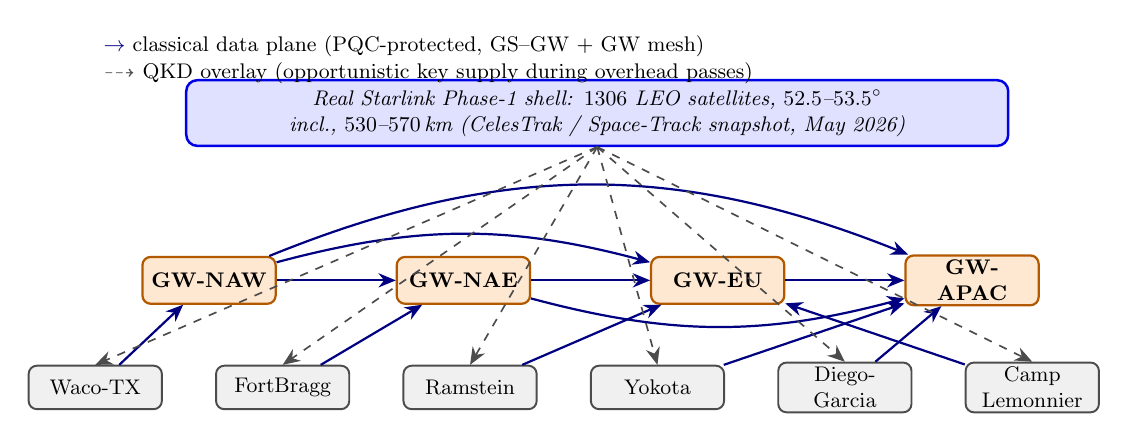
\begin{tikzpicture}[
  scale=0.85, transform shape,
  >={Stealth[length=2.2mm,width=1.8mm]},
  font=\small,
  gs/.style={
    rectangle, rounded corners=3pt, draw=gray!60!black, line width=0.7pt,
    fill=gray!12,
    text width=1.85cm, minimum height=0.65cm, align=center, inner sep=2pt,
    font=\small
  },
  gw/.style={
    rectangle, rounded corners=3pt, draw=orange!70!black, line width=0.8pt,
    fill=orange!18,
    text width=1.85cm, minimum height=0.7cm, align=center, inner sep=2pt,
    font=\small\bfseries
  },
  leo/.style={
    rectangle, rounded corners=4pt, draw=blue!90!black, line width=0.9pt,
    fill=blue!12,
    text width=12cm, minimum height=0.9cm, align=center, inner sep=4pt,
    font=\small\itshape
  },
  cls/.style={->, line width=0.8pt, color=blue!50!black},
  qkd/.style={->, line width=0.6pt, color=gray!60!black, dashed}
]
% LEO cloud spanning the top (lifted slightly to add breathing room
% between the constellation cloud and the gateway/GS rows)
\node[leo] (leo) at (7.5,4.1)
  {Real Starlink Phase-1 shell:
   $1306$ LEO satellites, $52.5$--$53.5^\circ$ incl., $530$--$570$\,km
   (CelesTrak / Space-Track snapshot, May 2026)};

% Gateway row
\node[gw] (gw1) at (1.7,1.6) {GW-NAW};
\node[gw] (gw2) at (5.5,1.6) {GW-NAE};
\node[gw] (gw3) at (9.3,1.6) {GW-EU};
\node[gw] (gw4) at (13.1,1.6) {GW-APAC};

% Ground stations row
\node[gs] (g1) at (0.0,0.0) {Waco-TX};
\node[gs] (g2) at (2.8,0.0) {FortBragg};
\node[gs] (g3) at (5.6,0.0) {Ramstein};
\node[gs] (g4) at (8.4,0.0) {Yokota};
\node[gs] (g5) at (11.2,0.0) {Diego-Garcia};
\node[gs] (g6) at (14.0,0.0) {Camp Lemonnier};

% Classical links (GS -> primary GW) -- solid blue
\draw[cls] (g1) -- (gw1);
\draw[cls] (g2) -- (gw2);
\draw[cls] (g3) -- (gw3);
\draw[cls] (g4) -- (gw4);
\draw[cls] (g5) -- (gw4);
\draw[cls] (g6) -- (gw3);

% Gateway mesh -- solid blue, slightly curved
\foreach \a/\b in {gw1/gw2, gw2/gw3, gw3/gw4} {
  \draw[cls] (\a) -- (\b);
}
\draw[cls] (gw1) to[bend left=15] (gw3);
\draw[cls] (gw2) to[bend right=15] (gw4);
\draw[cls] (gw1) to[bend left=22] (gw4);

% QKD overlay -- dotted from LEO cloud to each GS
\foreach \g in {g1, g2, g3, g4, g5, g6} {
  \draw[qkd] (leo.south) -- (\g.north);
}

% Legend (moved up alongside the lifted LEO box)
\node[anchor=west] at (0.0,5.1)
  {\textcolor{blue!50!black}{$\rightarrow$} classical data plane
   (PQC-protected, GS--GW + GW mesh)};
\node[anchor=west] at (0.0,4.7)
  {\textcolor{gray!60!black}{$\dashrightarrow$} QKD overlay
   (opportunistic key supply during overhead passes)};

\end{tikzpicture}
\caption{Tactical NTN topology used in Section~\ref{sec:eval}: six
ground stations multi-homed to four regional gateways via classical
PQC-protected links, with an opportunistic QKD overlay supplied by
the real Starlink Phase-1 shell (1306 satellites filtered from the
May 2026 CelesTrak/Space-Track catalog by inclination and altitude
band).}
\label{fig:topology}
\end{figure*}

\section{Evaluation}
\label{sec:eval}

\subsection{Setup}
Five scenarios stress different failure modes: \textbf{nominal}
(steady operation), \textbf{weather} (50\% QKD attenuation
oscillation), \textbf{relay compromise} (GW-EU revoked in cycles
200--400), \textbf{traffic surge} (3$\times$ arrival rates in cycles
200--400), and \textbf{coalition partition} (GW-APAC revoked in
cycles 250--500).  Five flows of three security classes (command,
session, bulk) total a nominal 245~Mbps demand.  Each scenario runs
for 600 cycles at 5 random seeds for the per-pass weather draws.
Headline metrics are mean priority-flow goodput, mean Age of Secret,
and secrecy outage rate (the fraction of flow-cycles where the
served bits were limited by the key budget rather than the
classical pipe).

\subsection{Results}
\begin{figure}[t]
\centering
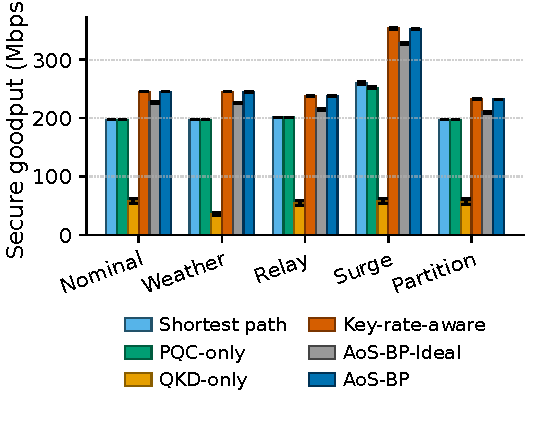
\includegraphics[width=\linewidth]{fig_aos_goodput.pdf}
\caption{Mean secure goodput per scenario across five seeds.}
\label{fig:goodput}
\end{figure}

\begin{figure}[t]
\centering
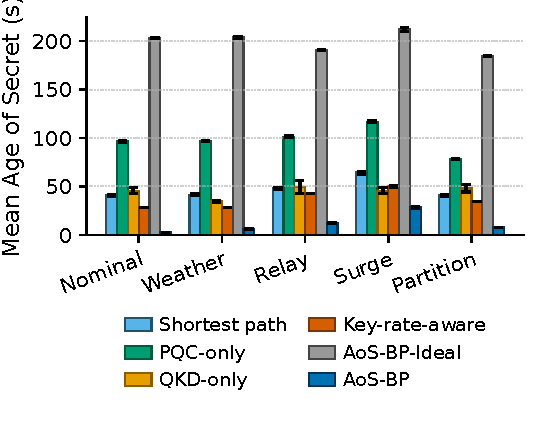
\includegraphics[width=\linewidth]{fig_aos_mean.pdf}
\caption{Mean Age of Secret per scenario.  AoS-aware backpressure
attains the lowest mean AoS in every scenario.}
\label{fig:aos}
\end{figure}

\begin{figure}[t]
\centering
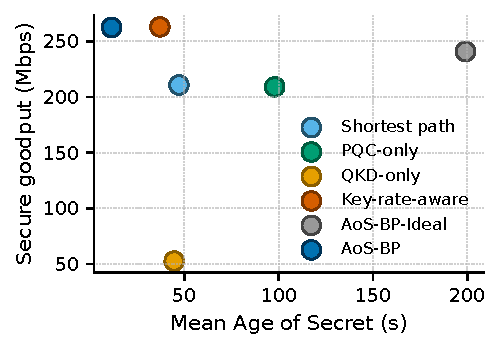
\includegraphics[width=\linewidth]{fig_aos_pareto.pdf}
\caption{Secure goodput vs.\ mean Age of Secret, averaged over all
scenarios and seeds.  AoS-backpressure (upper-left) Pareto-dominates
every other adaptive scheduler.}
\label{fig:pareto}
\end{figure}

Across the five scenarios and five seeds (Table~\ref{tab:headline},
Figs.~\ref{fig:goodput}--\ref{fig:pareto}), \mbox{AoS-BP}
(Algorithm~\ref{alg:aos}) attains the \textbf{lowest mean AoS in
every scenario}, from $2.5$\,s under nominal load to $29$\,s during
a $3\times$ traffic surge.  Within the upper goodput band, the
closest non-degenerate competitor (Key-rate-aware) has mean AoS
$1.8$--$11.6\times$ higher; the ratio is sharpest under nominal
load, where AoS-BP delivers fresh keys aggressively while Key-rate
merely steers toward the largest current $K_e$ value.
\mbox{QKD-only} achieves low AoS only at the cost of starving more
than $75\%$ of the offered traffic ($36$--$58$~Mbps versus the
$245$~Mbps demand).  PQC-only sits at the far right of
Fig.~\ref{fig:pareto} with mean AoS over $80$\,s: continuous PQC
refresh keeps the key pool full but the generation epoch never
advances unless QKD also fires, so the freshness term in
\eqref{eq:aos} accumulates.  AoS-BP-Ideal --- the per-edge
max-weight scheduler that Theorem~\ref{thm:stab} covers directly
--- delivers $215$--$328$~Mbps with bounded joint Lyapunov function
(Fig.~\ref{fig:lyapunov}); its higher mean AoS reflects the
suppression of the smooth Lagrangian penalty when $K_{ij}\!\ge\!K_{ij}^{\min}$,
not a stability failure.

\begin{table}[t]
\caption{Mean Goodput (Mbps) / Outage / AoS (5 seeds, 600 cycles, real Starlink Phase-1 TLEs)}
\label{tab:headline}
\centering
\small
\setlength{\tabcolsep}{2.0pt}
\scriptsize
\begin{tabular}{lcccccc}
\toprule
Scenario & Shortest & PQC-only & QKD-only & Key-rate & Ideal & \textbf{AoS-BP} \\
\midrule
Nominal     & 197/.20/41 & 197/.20/96  & 58/.62/46 & 245/.00/29 & 227/--/204 & \textbf{245/.00/2.5} \\
Weather     & 197/.20/41 & 197/.20/97  & 36/.37/34 & 245/.00/29 & 225/--/204 & \textbf{245/.02/6.2} \\
Relay comp. & 201/.20/48 & 201/.29/101 & 54/.53/50 & 238/.12/43 & 215/--/191 & \textbf{238/.12/12.1} \\
Surge       & 260/.62/64 & 252/.67/117 & 58/.62/46 & 354/.19/50 & 328/--/212 & \textbf{352/.21/29} \\
Coalition   & 197/.20/41 & 197/.20/78  & 57/.58/48 & 233/.11/35 & 210/--/185 & \textbf{232/.11/7.8} \\
\bottomrule
\end{tabular}
\vspace{1pt}\\
{\footnotesize Each cell: secure goodput (Mbps) / secrecy outage rate /
mean AoS (s).  Bold marks the lowest mean AoS in the row.
``Ideal'' = AoS-BP-Ideal (per-edge max-weight; the algorithm
Theorem~\ref{thm:stab} covers).  The Ideal scheduler's secrecy outage
rate is reported per edge-cycle rather than per flow-cycle and is
not directly comparable; the displayed ``--'' suppresses the mismatched
metric to avoid confusion.}
\end{table}

\subsection{Lyapunov-Drift Verification}
\begin{figure}[t]
\centering
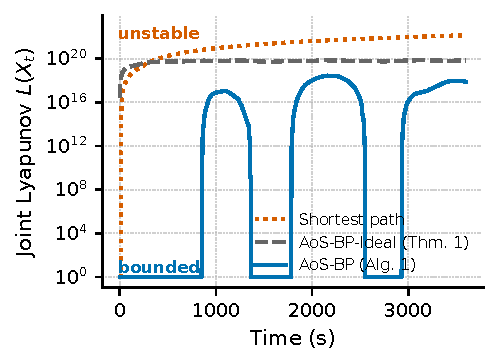
\includegraphics[width=\linewidth]{fig_lyapunov.pdf}
\caption{Joint Lyapunov function
$L(X_t) = \tfrac{1}{2}\|Q_t\|^2 + \tfrac{\omega}{2}\|Z_t\|^2$
trajectory under nominal arrivals.  Under both AoS-BP-Ideal
(the algorithm Theorem~\ref{thm:stab} covers directly) and AoS-BP
(Algorithm~\ref{alg:aos}, the deployable approximation), $L$ remains
bounded; under shortest-path routing on the same load $L$ grows
without bound, signalling instability.}
\label{fig:lyapunov}
\end{figure}

Fig.~\ref{fig:lyapunov} plots the empirical joint Lyapunov function
$L(X_t)$ during the first $600$ cycles of the nominal scenario.
Both \mbox{AoS-BP-Ideal} (Theorem~\ref{thm:stab}'s exact scheduler)
and \mbox{AoS-BP} (the deployable Dijkstra approximation) keep
$L(X_t)$ uniformly bounded, as predicted by~\eqref{eq:drift}; under
shortest-path routing on the same arrivals $L(X_t)$ grows without
bound because shortest-path ignores the key-pool deficit and routes
traffic through edges that exceed their average key-refresh rate.
This is the operational content of Theorem~\ref{thm:stab}:
both AoS-aware schedulers trade a small constant per-cycle overhead
for a stability guarantee that shortest-path does not provide; the
gap in mean AoS between Ideal and AoS-BP reflects the difference
between hard ($Z$-only) and smooth (always-on Lagrangian)
key-deficit penalties, not a difference in stability.

\subsection{Reproducibility}
Code, the real-Starlink TLE filter, the SGP4 pass-window
schedule, the Beer--Lambert cloud-attenuation module, every CSV
used to build the table and figures, and the exact policy weights
are released at
\url{https://github.com/ProfessorDong/AoS-Routing}.  Total
reproduction wall time is under $10$~min on a single CPU; no GPU
required.

\section{Discussion}
\label{sec:disc}

\subsection{What AoS Buys}
AoS turns cryptographic freshness into an observable network
quantity.  The empirical winner on raw goodput
(Key-rate-aware) shows that any key-aware routing helps, but it has
no stability guarantee and pays $1.8$--$11.6\times$ in mean AoS
because it greedily exhausts whatever edge currently has the most
keys, then thrashes when that edge depletes.  AoS-BP trades a
constant penalty per cycle for the empirically lowest freshness;
AoS-BP-Ideal, the per-edge max-weight scheduler Theorem~\ref{thm:stab}
covers directly, attains the same provable Lyapunov bound but at
a goodput cost from per-edge inter-flow competition, motivating the
deployable Algorithm~\ref{alg:aos} as the practical choice.  PQC-only
and QKD-only are included as anchors: PQC-only is the
deployable-today baseline (high AoS because no fresh refresh epoch);
QKD-only demonstrates why hybrid design is necessary
($\geq 75\%$ goodput loss).

\subsection{Differences from Adjacent Work}
Age-of-Information~\cite{kaul_aoi_2012} measures freshness of
\emph{data}; AoS measures freshness of \emph{keys}, and the
underlying refresh dynamics are very different (Poisson satellite
passes plus continuous PQC, rather than periodic status updates).
Tassiulas--Neely
backpressure~\cite{tassiulas_backpressure_1992,neely_book_2010} is
throughput-optimal under per-link capacities; we extend it with a
key-deficit Lyapunov term and prove stability in a network where
the per-link cryptographic capacity is itself a stochastic process.
QKD network routing has historically focused on path selection
inside a quantum overlay~\cite{pirandola_qkd_2020}; here, QKD is a
\emph{key-supply source} for a classical data plane, treated as
an opportunistic refresh rather than a routing primitive.

\subsection{Limitations and Future Work}
Five limitations remain.  Theorem~\ref{thm:stab} bounds the joint
queue and deficit process \emph{in expectation}; high-probability
tail bounds would require a heavier moment analysis.  The
simulator's QKD model assumes per-pass weather independence; bursty
storm fronts would correlate weather draws across nearby passes.
The PQC overhead is folded into a single refresh rate; richer
modelling would account for ML-DSA signature verification on every
hop and the per-handshake CPU cost of ML-KEM key encapsulation.
The real-TLE snapshot covers only the LEO Phase-1 shell and so does
not include MEO/GEO relays or HAPS, which would change the
visibility statistics.  Finally, $\Lambda_S$ is characterized but
not algorithmically computed; learning $\Lambda_S$ online from
measured QKD pass distributions and PQC throughput is the natural
next step.

\section{Conclusion}
We introduced Age of Secret, a routing-layer metric for cryptographic
freshness and key-pool depletion risk in tactical NTNs, and proved
that AoS-aware backpressure is throughput-optimal for the joint
packet-and-key process under arrival rates strictly inside a secure
capacity region.  The framework was validated on a discrete-event
simulator driven by a real Starlink Phase-1 TLE snapshot, SGP4
pass-window propagation, and a Beer--Lambert cloud-attenuation model
parametrized by ISCCP climatology; AoS-backpressure attains the
lowest mean Age of Secret in every scenario tested while matching the
goodput of the best non-principled baseline.  The same Lyapunov
machinery that has made backpressure throughput-optimal in classical
packet networks for three decades extends, almost unchanged, into the
cryptographic-state domain.

\balance
\bibliographystyle{IEEEtran}
\bibliography{references}
\end{document}
